\section[image=trams]{Two-phase commit}
\begin{frame}[plain]{}
    \sectionpage
\end{frame}

\begin{frame}
    \frametitle{Specifying two-phase commit}

    Our goal is to model a system with one \alert{transaction manager} and
    several \alert{resource managers} that need to perform a distributed
    transaction.
    The transaction may:
    \begin{itemize}
        \item \textbf{commit} if all resource managers have committed
        \item \textbf{abort} in any other case
    \end{itemize}

    \begin{center}
        \begin{tikzpicture}[
            >=stealth,
            edge from parent/.style={draw,<->},
            every node/.style={ellipse,draw}
        ]
            \node[rectangle, inner sep=.75em] (tm) {$tm$}
            child foreach \x in {rm1,rm2,rm3} {
                node {$\x$}
            };
        \end{tikzpicture}
    \end{center}
\end{frame}



\subsection{TCommit}
\begin{frame}
    \frametitle{Specifying transaction commit}
    We start with a simple setting, in which we only consider the
    \alert{resource managers} and their \alert{states}.
    We do \emph{not} model
    \begin{itemize}
        \item the transaction manager
        \item the communication channels
        \item the transaction itself
    \end{itemize}
    \uncover<2->{
    We write the specification in module $TCommit$, which will be refined later

    \begin{center}
        \begin{tlatex}
            \moduleLeftDash{ {\MODULE} $TCommit$}\moduleRightDash
        \end{tlatex}
    \end{center}
    }
\end{frame}

\setbeamercovered{transparent}

\begin{frame}
    \frametitle{Constants and variables}

    We declare $RM$ as the set of all resource managers and $rmState$ as the
    state of each resource manager.
    \begin{tlabox}
        &\CONSTANT RM \\
        &\VARIABLE rmState
    \end{tlabox}

    Every constant value is a set -- even 0, 1 and the string "xyz" --
    but for the former their elements are simply undefined, so we
    can't test if $a \in 0$.

    We will assign elements to $RM$ when performing model checking.
\end{frame}

\begin{frame}
    \frametitle{Type checking}
    \begin{uncoverenv}<1>
        \tlap doesn't provide explicit typing of variables. It is customary to
        define an invariant $TypeOK$ to specify the \alert{domain} of each variable.
    \end{uncoverenv}
    \begin{uncoverenv}<2>
        We specify that $rmState$ is an array indexed by $RM$ with values in
        the set of strings below.
    \end{uncoverenv}
    \begin{uncoverenv}<2->
        \begin{tlabox}
            TCTypeOK \defeq rmState \in
            [RM \rightarrow \{&\str{working}, \str{prepared}, \\
                            &\str{committed},\str{aborted}\}]
        \end{tlabox}
    \end{uncoverenv}
    \begin{uncoverenv}<3>
        You can think of it as a mathematical function
        \[
            rmState: RM \rightarrow \{\str{working}, \dots\}
        \]
        We can refer to a value with $rmState[r]$, where $r \in
        RM$.
    \end{uncoverenv}
\end{frame}

\begin{frame}
    \frametitle{The temporal formula of the specification}
    \begin{uncoverenv}<1->
            We specify the behavior with a temporal formula
        \begin{tlabox}
            TCSpec \defeq TCInit \land \Box [TCNext\,]_{rmState}
        \end{tlabox}
    \end{uncoverenv}
    \begin{uncoverenv}<1->
        where initially each resource manager is working
        \begin{tlabox}
            TCInit \defeq [ r \in RM \mapsto \str{working}]
        \end{tlabox}
        and at each step either all resource managers remain in their
        current state (stuttering step) or they take a $Next$-step
    \end{uncoverenv}
\end{frame}

\begin{frame}
    \frametitle{Evolution of the system}

    \begin{columns}[c]
    \begin{column}{0.65\textwidth}
        \uncover<1>{What is a possible step of our system?}

        \uncover<2,3>{A resource manager may}
        \begin{itemize}
            \item<2> Finish working and become prepared
            \item<3> Decide to commit or abort
        \end{itemize}
    \end{column}
    \begin{column}{0.35\textwidth}
        \centering
        \scalebox{.75}{
            \begin{tikzpicture}[
                >=stealth,
                sibling distance=7em,
                edge from parent/.style={draw,->},
                every node/.style={ellipse,draw}
            ]
                \node (w) {$working$}
                child {
                    node (p) {$prepared$}
                    child {
                        node[inner xsep=0] (c) {$committed$}
                    }
                    child {
                        node (a) {$aborted$}
                    }
                };
                \path [draw, ->] (w.south east) to [bend left=30] (a.north);
            \end{tikzpicture}
        }
    \end{column}
    \end{columns}
    \vspace{\baselineskip}
    \begin{tlabox}
        TCNext \defeq \uncover<2,3>{\E r \in RM :}
        \uncover<2>{Prepare(r\,)} \uncover<3>{\lor Decide(r\,)}
    \end{tlabox}
\end{frame}

\begin{frame}
    \frametitle{The Prepare action}

    Resource manager $r$ evolves from \str{working} to \str{prepared},
    while all the other ones remain in the same state.
    \begin{tlabox}
        Prep&are(r) \defeq \\
            &\uncover<1>{%
            \land rmState[r\,] = \str{working}} \\
            &\uncover<2>{%
            \land rmState' = [rmState \EXCEPT \bang[r\,] = \str{prepared}]}
    \end{tlabox}

\end{frame}

\begin{frame}
    \frametitle{The Decide action}

    \only<1>{%
    First subformula: transition \alert{$prepared \rightarrow committed$}}
    \only<2>{%
    Second subformula: transition \alert{$working, prepared \rightarrow aborted$}}
    \begin{tlabox}
        De&cide(r) \defeq \\
            &\lor \uncover<1>{%
                \land rmState[r\,] = \str{prepared}} \\
            &\phantom{\.{\lor}} \uncover<1>{%
                \land canCommit} \\
            &\phantom{\.{\lor}}\uncover<1>{%
                \land rmState' = [rmState \EXCEPT \bang[r\,] = \str{committed}]} \\
            &\lor \uncover<2>{%
                \land rmState[r\,] \in \{\str{working}, \str{prepared}\}} \\
            &\phantom{\.{\lor}}\uncover<2>{
                \land notCommitted} \\
            &\phantom{\.{\lor}}\uncover<2>{%
                \land rmState' = [rmState \EXCEPT \bang[r\,] = \str{aborted}]}
    \end{tlabox}

    \begin{onlyenv}<1>
        \begin{tlabox}
            canCommit \defeq \A r \in RM : rmState[r\,] \in \{\str{prepared},
            \str{comm.}\}
        \end{tlabox}
    \end{onlyenv}

    \begin{onlyenv}<2>
        \begin{tlabox}
            notCommitted \defeq \A r \in RM : rmState[r\,] \neq \str{committed}
        \end{tlabox}
    \end{onlyenv}

\end{frame}

\begin{frame}
    \frametitle{Checking the specification}

    Once we have modeled how the system \emph{behaves}, we can use TLC to check
    if desired properties hold.

    In particular we are interested in checking that \alert{no two RMs have
    arrived at conflicting decisions}. This \emph{safety property} can be
    expressed with the invariant $TCConsistent$:

    \begin{tlabox}
        TC&Consistent \defeq \\
        &\A r1, r2 \in RM : \neg
            \land rmState[r1] = \str{aborted} \\
        &\phantom{\A r1, r2 \in RM : \.{\neg}}
            \land rmState[r2] = \str{committed}
    \end{tlabox}

\end{frame}

\subsection{TwoPhase}

\begin{frame}
    \frametitle{Refining the specification}

    Now we create module $TwoPhase$ where we refine our specification,
    adding the following variables
    \begin{itemize}
        \item $tmState$ -- control state of the tr. manager (init or done)
        \item $tmPrepared$ -- set of r.m.s that t.m. knows are prepared
        \item $msgs$ -- set of all messages ever sent
    \end{itemize}

    while $rmState$ is defined as in the previous module.

    \begin{center}\scalebox{.75}{
        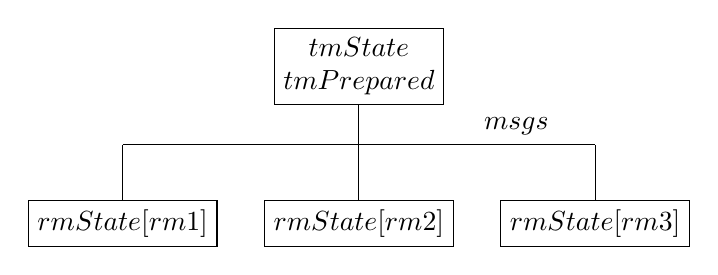
\begin{tikzpicture}[
            >=stealth,
            ent/.style={draw, rectangle, align=center},
            pnt/.style={circle, fill, inner sep=0.15em}
        ]
           \node[ent] at (0,2)(tm) {$tmState$ \\ $tmPrepared$};


           \node[ent] (rm1) at (-3,0) {$rmState[rm1]$};
           \node[ent] (rm2) at (0,0) {$rmState[rm2]$};
           \node[ent] (rm3) at (3,0) {$rmState[rm3]$};

           \draw (-3,1) -- (0,1) -- (3,1);
           \draw (rm1) -- (-3,1);
           \draw (rm2) -- (tm);
           \draw (rm3) -- (3,1);
           \node[above] (msgs) at (2,1) {$msgs$};
        \end{tikzpicture}
    }\end{center}

\end{frame}

\begin{frame}
    \frametitle{Refining the specification}

    The specification for this model is
    \begin{tlabox}
        TPSpec \defeq TPInit \land \Box [TPNext\,]_{\langle
        rmState,\, tmState,\, tmPrepared,\, msgs \rangle}
    \end{tlabox}

    Now we want to check if $TPSpec$ implements $TCSpec$, so we import the
    definitions from module $TCommit$
    \begin{tlabox}
        \INSTANCE TCommit \textcolor{gray!50}{\WITH rmState \leftarrow rmState}
    \end{tlabox}
    and check that \alert{$TPSpec \implies TCSpec$} with TLC.

    \begin{center}
        \scriptsize
        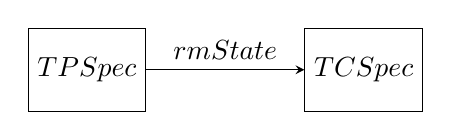
\begin{tikzpicture}[
            >=stealth,
            block/.style={draw, rectangle,
                            minimum height=3em, minimum width=3em}
        ]

            \node[block] (tp) {$TPSpec$};
            \node[block, right of=tp, node distance=10 em] (tc) {$TCSpec$};

            \draw[draw,->] (tp) -- node[above] {$rmState$} (tc);

        \end{tikzpicture}
    \end{center}

\end{frame}

\begin{frame}
    \frametitle{A common step}

    \begin{tlabox}
        TPSpec \defeq TPInit \land \Box [TPNext\,]_{\langle
        rmState,\, tmState,\, tmPrepared,\, msgs \rangle}
    \end{tlabox}

    {\scriptsize
    \setlength\abovedisplayskip{0pt}
    \setlength\belowdisplayskip{0pt}
    \begin{alignat*}{2}
        &\begin{bmatrix}
            tmState : \str{init} \\
            tmPrepared : \{\} \\
            msgs : \{\} \\
            rmState[rm1] : \str{work.}
        \end{bmatrix}
        &\xrightarrow{RMPrepare(rm1)}&
        \begin{bmatrix}
            tmState : \str{init} \\
            tmPrepared : \{\} \\
            \alert{
            msgs = \{[type :\str{Prep}, rm : rm1]\}} \\
            \alert{
            rmState[rm1] : \str{prep.}}
        \end{bmatrix}
        \\[\baselineskip]
        &\begin{bmatrix}
            rmState[rm1] : \str{work.} \\
        \end{bmatrix}
        &\xrightarrow{\phantom{R}Prepare(rm1)\phantom{M}}&
        \begin{bmatrix}
            \phantom{msgs \ \ }
            \alert{
            rmState[rm1] : \str{prep.}}
            \phantom{msgs \ \ }
        \end{bmatrix}
    \end{alignat*}
    }

    \begin{tlabox}
        TCSpec \defeq TCInit \land \Box [TCNext\,]_{rmState}
    \end{tlabox}

\end{frame}

\begin{frame}
    \frametitle{A stutter step}

    \begin{tlabox}
        TPSpec \defeq TPInit \land \Box [TPNext\,]_{\langle
        rmState,\, tmState,\, tmPrepared,\, msgs \rangle}
    \end{tlabox}

    {\scriptsize
    \setlength\abovedisplayskip{0pt}
    \setlength\belowdisplayskip{0pt}
    \begin{alignat*}{2}
        &\begin{bmatrix}
            tmState : \str{init} \\
            tmPrepared : \{\} \\
            msgs = \{\dots\} \\
            rmState[rm1] : \str{prep.}
        \end{bmatrix}
        &\xrightarrow{TMRcvPrepared(rm1)}&
        \begin{bmatrix}
            tmState : \str{init} \\
            \alert{
            tmPrepared : \{rm1\}} \\
            msgs : \{\dots\} \\
            rmState[rm1] : \str{prep.}
        \end{bmatrix}
        \\[\baselineskip]
        &\begin{bmatrix}
            rmState[rm1] : \str{prep.}
        \end{bmatrix}
        &\xrightarrow{\phantom{T} \UNCHANGED rmState \phantom{T}}&
        \begin{bmatrix}
            rmState[rm1] : \str{prep.} \\
        \end{bmatrix}
    \end{alignat*}
    }

    \begin{tlabox}
        TCSpec \defeq TCInit \land \Box [TCNext\,]_{rmState}
    \end{tlabox}

\end{frame}

\begin{frame}
    \frametitle{Taking advantage of symmetry}

    TLC is an explicit-state model checker, so it suffers from state
    explosion. Consider the following possible states according to $TPSpec$:

    {\setlength\abovedisplayskip{0pt}
    \setlength\belowdisplayskip{0pt}
    \begin{gather*}
        s =
        \begin{bmatrix}
            rmState[\textcolor{redPolimi}{rm1}] : \str{prep.} \\
            rmState[\textcolor{bluePolimi}{rm2}] : \str{prep.} \\
            rmState[\textcolor{yellowPolimi}{rm3}] : \str{com.} \\
            \dots
        \end{bmatrix}
        \quad
        s^{\pi} =
        \begin{bmatrix}
            rmState[\textcolor{yellowPolimi}{rm3}] : \str{prep.} \\
            rmState[\textcolor{bluePolimi}{rm2}] : \str{prep.} \\
            rmState[\textcolor{redPolimi}{rm1}] : \str{com.} \\
            \dots
        \end{bmatrix} \\
        \pi = [
            rm1 \mapsto rm3,\,
            rm2 \mapsto rm2,\,
            rm3 \mapsto rm1
        ]
    \end{gather*}}

    Since permutations such as $\pi$ are irrelevant for us, we can take
    advantage of \emph{symmetry}.

\end{frame}

\begin{frame}
    \frametitle{Taking advantage of symmetry}

    \begin{block}{Symmetric specification}
        \setlength\belowdisplayskip{0pt}
        A specification $Spec$ is symmetric with respect to a permutation $\pi$
        over a set of values $S$ if and only if for each behavior $\sigma$:
        \[
             \sigma \models Spec \iff \sigma^{\pi} \models Spec
        \]
    \end{block}

    $TPSpec$ is indeed symmetric w.r.t. the permutations of set $RM$,
    since all resource managers are equal.

    After stating that \alert{$RM$ is a symmetry set} in our model, if TLC
    has already visited a state $s$, it will avoid visiting a state $s^{\pi}$,
    where $\pi$ is a permutation of values in $RM$.

    A reduction of a factor $\lvert RM \rvert !$ can be observed for the number
    of states to be checked.

\end{frame}

\setbeamercovered{invisible}
